%% LyX 2.2.4 created this file.  For more info, see http://www.lyx.org/.
%% Do not edit unless you really know what you are doing.
\documentclass[american,twocolumn]{bmcart}
\usepackage[T1]{fontenc}
\usepackage[utf8]{inputenc}
\setcounter{secnumdepth}{3}
\setcounter{tocdepth}{3}
\usepackage{float}
\usepackage{graphicx}

\makeatletter
%%%%%%%%%%%%%%%%%%%%%%%%%%%%%% User specified LaTeX commands.
\usepackage{paperBMC_preamble}

\makeatother

\usepackage{babel}
\begin{document}
\begin{frontmatter}
\begin{fmbox}
\dochead{Research}

\title{A fast parallel algorithm to reduce protein folding trajectories}

\maketitle
\author[
   addressref={aff1},                   % id's of addresses, e.g. {aff1,aff2}   
   email={lgarreta@agrosavia.co}   % email address
]{\inits{LG}\fnm{Luis} \snm{Garreta}}
\author[
   addressref={aff2},
   email={mmartinez@ebi.ac.uk}
]{\inits{MM}\fnm{Mauricio} \snm{Martinez}}
\author[
   addressref={aff3},
   email={nediaz@unicauca.edu.co}
]{\inits{ND}\fnm{Néstor A} \snm{Díaz}}
\author[
   addressref={aff4},
   corref={aff4},                       % id of corresponding address, if any
   email={pedro.moreno@correounivalle.edu.co}
]{\inits{PM}\fnm{Pedro A} \snm{Moreno}}

%%%%%%%%%%%%%%%%%%%%%%%%%%%%%%%%%%%%%%%%%%%%%%%%%%%%%%%%
\address[id=aff1]{%                           % unique id
  \orgname{Corporaci\'{o}n Colombiana de Investigaci\'{o}n Agropecuaria - AGROSAVIA, CI Tibaitat\'{a},  Kil\'{o}metro 14, V\'{i}a a Mosquera, 250047, Colombia}, % university, etc
  %\street{},                     %
  %\postcode{}                                % post or zip code
  \city{Santiago de Cali},                              % city
  \cny{Colombia}                                    % country
}
\address[id=aff2]{%
  \orgname{The European Bioinformatics Institute (EMBL-EBI)},
  %\street{D\"{u}sternbrooker Weg 20},
  %\postcode{24105}
  \city{Hinxton, Cambridgeshire},
  \cny{UK}
}
\address[id=aff3]{%                           % unique id
  \orgname{Facultad de Ingeniería Electrónica y Telecomunicaciones,  Universidad del Cauca}, % university, etc
  %\street{},                     %
  %\postcode{}                                % post or zip code
  \city{Popayán},                              % city
  \cny{Colombia}                                    % country
}
\address[id=aff4]{%                           % unique id
  \orgname{Escuela de Ingeniería de Sistemas y Computación, Universidad del Valle}, % university, etc
  %\street{},                     %
  %\postcode{}                                % post or zip code
  \city{Santiago de Cali},                              % city
  \cny{Colombia}                                    % country
}

\begin{artnotes}
\note[id=n1]{Equal contributor} % note, connected to author
\end{artnotes}


%\end{fmbox}% comment this for two column layout
\begin{abstractbox}
\begin{abstract}
\parttitle{Background} Simulations are among the most important tools for studying the mechanisms underlying protein folding. Protein folding simulations have experienced substantial progress in recent years. Diverse technologies are employed, and simulations are reaching the microsecond timescale and greater, which generate very long trajectories. However, the analysis of these trajectories is complicated, and tools are necessary to simplify them so that both the main events and the temporal order in which they occur are preserved.

\parttitle{Results} We present an algorithm to reduce long protein-folding trajectories in a fast and parallel way. The algorithm divides a trajectory into segments to be processed in parallel and then selects from each segment the most representative conformations using a rapid clustering strategy. This strategy leverages the temporal order of the conformations to compare them locally, avoiding an all-versus-all comparison. The algorithm reduces a trajectory by a high percentage, preserving both the patterns and the structure obtained by other, more complex reduction techniques. In addition, its performance is close to that of other efficient reduction techniques and is improved when executed in parallel using more than one core.

\parttitle{Conclusions} The proposed algorithm quickly reduces a protein folding trajectory by selecting its most representative conformations and preserves both the structure and temporal order of the trajectory. The reduced trajectories can be used as input for more complex analysis techniques and for other reduction techniques that are impractical for use with long folding trajectories. The algorithm is fast and is designed to run in parallel on conventional PCs with multicore technology, which are present in most typical research laboratories.
\end{abstract}
\begin{keyword}
\kwd{Protein folding simulations}
\kwd{Protein structure comparison}
\kwd{Protein structure clustering}
\end{keyword}

\end{abstractbox}
\end{fmbox}% uncomment this for two column layout 
\end{frontmatter}

\section*{Background}

We present a parallel algorithm to reduce protein folding trajectories that quickly obtains representative conformations, conserving both the three-dimensional (3D) structure and temporal order of the trajectories. Proteins play fundamental roles in all living organisms, but to be functional, they must fold from their linear amino acid (AA) sequence into a unique 3D or native state; this process is known as protein folding. Understanding the mechanisms and rules of this process has been one of the most pursued objectives of computational biology, and an important theoretical tool to study these phenomena is simulation. Simulations are used to generate folding trajectories (Figure \ref{fig:Folding-Trajectory}), which describe the sequence of states that proteins follow as a function of time during the folding process.

\begin{figure}[th]
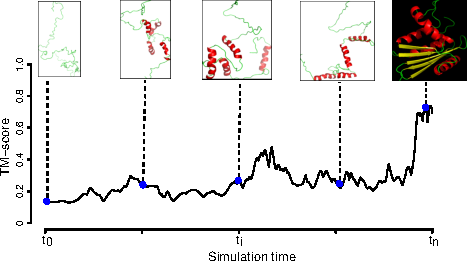
\includegraphics[bb=0bp 0bp 224bp 125bp]{images/01-trajectory-description-2RN2-pdbs}

\caption{\csentence{Protein folding trajectory.} Some protein conformations with their three-dimensional structure are marked as blue dots along the trajectory. The evolution of folding is measured at each step by comparing the structure at time $t_{i}$ to the native structure (black image background) using a structure comparison metric; in this work, we use the TM-score as the metric (see Methods). X-axis: Simulation time from $t_{0}$ to $t_{n}$. Y-axis: TM-score value from 0 (different) to 1 (similar). \label{fig:Folding-Trajectory}. }
\end{figure}

Most folding simulations use the molecular dynamics (MD) method, which, due to its computational cost, is limited to small proteins (<100 AA) and very short times (picoseconds or microseconds). However, technological innovations have allowed significant advances in these simulations, both with respect to time scale and the technology employed to execute them.

In 2011, using the Anton supercomputer, specifically designed for protein folding \cite{Shaw2008}, full simulations of 12 proteins were published, several on the order of milliseconds \cite{Shaw2011}. And more recently, in 2020, several trajectories related to the study of the SARS-Cov2 virus were released by DE Shaw Research \cite{Shaw2020}. The trajectories, on the order of microseconds, were simulated on Anton 2 {[}\#Shaw2014{]}, a supercomputer up to ten times faster than its predecessor Anton. As an economic alternative, in 2014, graphic processing units (GPU) were used to simulate the folding of 17 proteins on the order of microseconds, \cite{Nguyen2014}. And years earlier, in 2007, the Folding@home distributed computing platform utilized as many as 250,000 PCs, voluntarily available around the world, to simulate on the order of microseconds the folding of the villin-headpiece protein \cite{Larson2009}.

These innovations have allowed significant progress in protein folding simulations, both with respect to time scale and the technology used to execute them, resulting in the generation of trajectories with millions of conformations. However, due to the large number of conformations, their processing and analysis with conventional PCs is computationally expensive, and new algorithms are needed to simplify them while preserving as much information as possible.

Two approaches that have been used to reduce protein folding trajectories are dimensionality reduction \cite{Duan2013} and clustering \cite{Peng2018}. In the dimensionality reduction approach, conformations are transformed into reduced sets of variables that represent the original conformations as well as possible. Both linear and non-linear techniques have been used (e.g., principal component analysis (PCA) and multidimensional scaling \cite{RajanSchulten10}, Isomap \cite{Das2006}, diffusion maps \cite{Kim2015}). However, the reductions produced by these techniques lose the structural information of the conformations (Figure \ref{fig:lost-info-dimensionality}, top), and their interpretation becomes difficult since the new dimensions lack a clear relationship with the initial folding trajectory \cite{Cavallo2018}.

In the clustering approach, the conformations are assigned to groups that share similar characteristics (e.g., similarity with the native structure), and from each group, an average representative or its general characteristics can be obtained. Hierarchical and partitioned clustering have been used for this approach (e.g., k-means \cite{Doerr2017}, link \cite{Shao2007}). However, the groups lose their temporal order since they can include conformations that occur in very distant times (Figure \ref{fig:lost-info-dimensionality}, bottom).

In addition, the techniques of both approaches often require pair-wise comparisons, which are computationally costly when the trajectories are very large.

\begin{figure}[th]
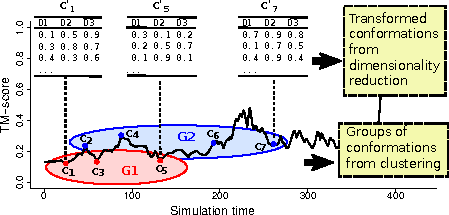
\includegraphics[bb=0bp 0bp 210bp 104bp,scale=1.05]{images/02-2RN2-trajectory-weakness}

\caption{\csentence{Loss of information in dimensionality reduction and clustering.} The dimensionality reduction method (above) transforms the conformations ( $c_{1},c_{5}$, and $c_{7}$) into a new set of values ( $c'_{1},c'_{5}$, and $c'_{7}$), but their structural information is lost, whereas the clustering method (bottom) forms two groups (G1 and G2), but their temporal order is lost since they contain conformations that overlap in time ($c_{2},c_{3},c_{4},c_{5}$). \label{fig:lost-info-dimensionality}}
\end{figure}

To reduce a folding trajectory, the proposed algorithm divides the path into segments that are processed in parallel. For each segment, characteristic events are quickly extracted using the rapid clustering strategy of Hobohm and Sander (1992) adapted here for protein folding trajectories. From these results, the most representative events are selected by a strategy of k-medoids \cite{Kaufman1990}. The results of each segment are joined to form the reduced trajectory with the most representative conformations of the original trajectory while retaining both its 3D representation and temporal order.

The algorithm is implemented in the R language except for the function used for pairwise structure comparison, the TM-score \cite{Zhang2004}, this function is executed many times and is implemented in the Fortran language.

\section*{Methods}

\subsection*{Datasets of protein folding trajectories}

We used the folding trajectories of three proteins obtained from different simulation projects. One of the trajectories was that of the trp-cage protein (PDB: 2JOF), simulated with MD using the Anton supercomputer \cite{Shaw2011}, with a simulation time of 208 \us, a time step of 200 \ps, and 1044001 conformations. The second trajectory was that of the apo papain-like protease of SARS-CoV-2 (6WX4), simulated with MD using the Anton 2 supercomputer \cite{Shaw2020}, with a simulation time of 100 \us, a time step of 1 \ns, and 100000 conformations. And the third trajectory was that of the villin-headpiece protein (2F4K), also simulated with MD using the Folding@home distributed platform \cite{PandeEnsign07}, with a simulation time of 8 \us, a time step of 50 \ps, and 15201 conformations. 

\subsection*{Time steps and folding steps}

A time step in MD trajectories is the time length at which conformations are sampled or evaluated during the simulation, whereas a folding step, as employed in the reduced trajectories produced by our algorithm, represents the most likely conformation occurring during a time interval or from a set of likely candidate conformations.

\subsection*{Pairwise comparison of protein structures using the TM-score \label{sec:Comparing-Structures}}

In this work, we used the TM-score metric for the pairwise comparison of protein structure \cite{Zhang2004}. This metric is used in both the proposed algorithm and in the techniques for reduction of protein folding used for benchmarking the algorithm against existing methods. The TM-score is more sensitive to the global topology than local variations; thus, it estimates the pairwise similarity of protein structures much more accurately than the Root Mean Square-Deviation (RMSD), a common metric used for the same purpose. The TM score between two structures ranges from 0 to 1, where 1 is a perfect match. According to a previous analysis \cite{zhang2010}, a TM score below 0.17 indicates no similarity between the two structures, while a TM score above 0.5 indicates a degree of similarity between them beyond what is expected by chance.

\subsection*{Other techniques for protein folding reduction \label{subsec:Techniques-for-reduction}}

nMDS and clustering techniques were used to obtain the intrinsic information of both the original and reduced trajectories, and their results were compared (see Results).

nMDS reductions were carried out using the R-function monoMDS \cite{Oksanen2019}, taking as input the dissimilarity matrix obtained from the pairwise comparisons of all the protein conformations of the folding trajectory. The complete-linkage clustering reductions were carried out using the R-function hclust \cite{RCoreTeam2018}, taking as input a matrix with the first two principal components from a PCA analysis. This PCA analysis was carried out using the R-function pca.xyz \cite{Grant2006}, taking as input a matrix with the 3D coordinates of the $C\alpha$ atoms of all the protein conformations of the folding trajectory.

The reduced trajectories were calculated with our algorithm from the villin-headpiece trajectory with 15201 conformations \cite{Larson2009}. The first reduced trajectory had 7197 conformations (representing a reduction of 52\%), and the second had 2258 conformations (representing a reduction of 80\%).

\section*{Implementation}

The proposed algorithm reduces a trajectory of protein folding in three steps: partitioning, extraction, and selection. The first step runs only once, whereas the other two runs several times independently, allowing them to run in parallel. Each step involves a strategy to improve the efficiency of the algorithm when working with large protein-folding trajectories. Figure \ref{fig:Algorithm-Description} shows the overview of the algorithm, and the steps are given below.

\begin{figure}[th]
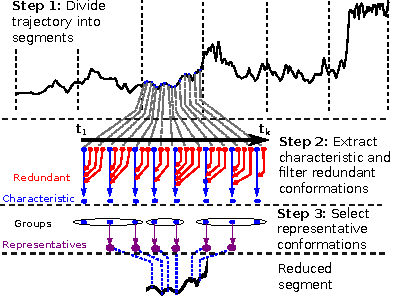
\includegraphics[scale=1.2]{images/03-algorithm-description-general}

\caption{\csentence{Overview of the proposed algorithm.} Step 1: Divide the trajectory into segments (vertical dashed lines) and reduce each individually. Each segment has $k$ conformations from time $t_{1}$ to $t_{k}$. Step 2: For each segment, extract characteristic conformations (blue dots) and remove redundant ones (red dots). Step 3: Select the most representative conformations among the previous conformations to obtain a reduced segment. \label{fig:Algorithm-Description}}
\end{figure}


\subsection*{Step 1: Partitioning}

In step 1, the trajectory is divided into segments to reduce them locally and in parallel (dotted vertical lines, Figure \ref{fig:Algorithm-Description}). This process is carried out by dividing the trajectory from the start to the end in segments with $k$ conformations each, where $k$ is an input parameter for the algorithm. Local reductions allow focus on the particular characteristics of each segment that will determine the global characteristics of the trajectory. The parallel reductions allow improved algorithm efficiency when it runs on machines with more than one processor (e.g., multicore computers) (Figure \ref{fig:Algorithm-Parallel}).

\begin{figure}[th]
\begin{centering}
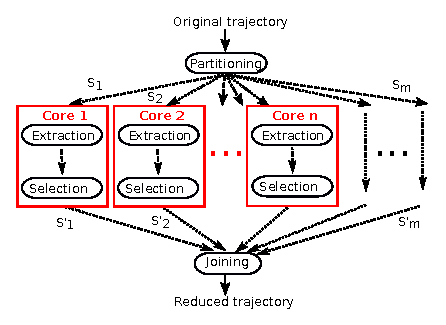
\includegraphics{images/04-algorithm-description-parallel}
\par\end{centering}
\caption{\csentence{Parallel processing of segments.} The trajectory is divided into $m$ segments ($S_{1}$, ..., $S_{m}$), and each segment is processed separately and in parallel on a machine with n processing cores. The results of the extraction and selection steps ($S'_{1}$, ..., $S'_{m}$) are independent of each other and are joined to form the reduced trajectory.\label{fig:Algorithm-Parallel}}
\end{figure}


\subsection*{Stage 2: Extraction}

In step 2, the characteristic conformations of each segment are rapidly extracted, and the redundant ones are eliminated. This step is efficiently carried out by means of a rapid clustering approach that performs few pairwise comparisons and extracts the most dissimilar conformations of a segment instead of grouping similar ones.

Here, we improved the fast clustering algorithm of Hobohm and Sander (1992) to work with a trajectory segment and exploit the implicit order of its conformations given by its simulation time (black horizontal line, Figure \ref{fig:Algorithm-Description}). Our algorithm selects the initial conformation at time $t_{1}$~as the first characteristic. Then, it compares this characteristic with the next conformation. If dissimilar, the last conformation becomes a new characteristic; otherwise, the last conformation is redundant and is removed (red dots, Figure \ref{fig:Algorithm-Description}). The process continues with the remaining conformations until finishing with the final one at time $t_{k}$, thus producing the set of representative characteristics of the segment (purple dots, Figure \ref{fig:Algorithm-Description})

\subsection*{Step 3: Selection}

In step 3, the conformations of the previously extracted characteristics are clustered to select the most representative characteristics. To identify these representatives, the algorithm uses a k-medoids strategy (PAM algorithm \cite{Kaufman1990}) that calculates the k conformations (medoids) with the minimal average difference between all the other members of the group.

The PAM algorithm needs as input a dissimilarity matrix with the pairwise comparisons of all-versus-all conformations of the trajectory segment; generating this matrix is an intensive computational task when the number of conformations is very large. However, this task is feasible here since the algorithm is working with a reduced set of characteristic conformations (attained in the previous step) of a trajectory segment and not the complete trajectory.

\section*{Results and Discussion}

Three tests were carried out to evaluate the capacity and performance of the proposed algorithm. In the first test, reduction of three trajectories was performed using the proposed algorithm. In the second, the intrinsic information preserved by the reductions was compared between our algorithm and two other folding reduction techniques. In the third, the performance of the methods was compared. 

\subsection*{Reduction of protein folding trajectories}

Figure \ref{fig:Trajectory-Results} shows the TM-score plots of the reduced trajectories produced by the proposed algorithm. The plots show that the algorithm attempts to find the most representative conformations from the original trajectories while conserving two fundamental properties: the structure and the temporal ordering of the original conformations. The other folding reduction methods investigated lose these properties in their reductions, as described in the next section.

As a result, these reduced trajectories become a summary of the original ones and can be used as inputs for more complex analyses or other reduction methods that require pairwise comparisons but are impractical for large trajectories.

\begin{figure*}[!t]
\begin{centering}
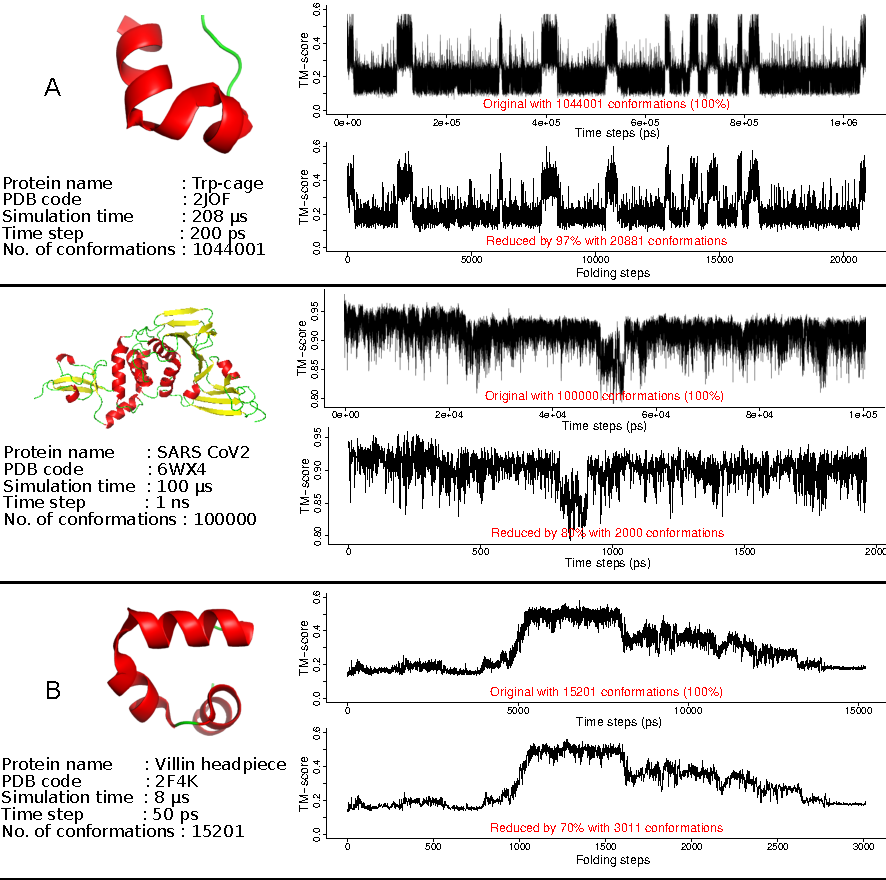
\includegraphics{images/05-path-comparisons}
\par\end{centering}
\caption{\csentence{Plots of the TM-score values for the original and reduced trajectories.} Protein and simulation details on the left. Trajectories on the right: original (upper part), and reduced (lower part). (A) Trajectory of trp-cage protein, reduced by 98\%, from 1044001 to 20881 conformations. (B) Trajectory of SARS CoV2 protein, reduced by 80\%, from 100000 to 2000 conformations. (C) Trajectory of the villin-headpiece protein, reduced by 80\%, from 15201 to 3011 conformations. \label{fig:Trajectory-Results}}
\end{figure*}


\subsection*{Comparison with other methods \label{sec:Comparing-other-methods}}

We compared how the intrinsic information captured from a folding trajectory by other folding reduction techniques is also preserved in the reductions produced by our algorithm. First, two reduced trajectories were computed from the original trajectory of the villin-headpiece protein using our algorithm, and then the intrinsic information was computed on these trajectories using nMDS and clustering reductions (Figure \ref{fig:Comparaciones-PCA-nMDS}) (see Methods for the details of the trajectory and techniques).

As shown in Figure \ref{fig:Comparaciones-PCA-nMDS}, the pattern of circles of points from nMDS and the structure of the three groups from clustering are consistent between the original and reduced trajectories. This result shows that the reductions produced by the proposed algorithm largely preserve the intrinsic information observed in the original trajectory. Furthermore, the proposed algorithm has several advantages. First, contrary to nMDS and clustering, our algorithm avoids the calculation of the dissimilarity matrix, which is a computationally expensive task for medium to large trajectories. Second, its reductions are a set of protein conformations, in contrast to the transformations produced with other techniques, such as nMDS, PCA, Isomap or diffusion maps \cite{RajanSchulten10,Duan2014,Kim2015}, which, in addition to losing the structural information of the conformations, the reductions can only be interpreted with the knowledge or experience in the intrinsic algorithm used by the technique \cite{Cavallo2018}.

Third, in the proposed algorithm, the temporal ordering of conformations is conserved, in contrast to clustering methods \cite{Peng2018} that merge configurations from different simulation times into clusters.

\begin{figure}[!th]
\begin{centering}
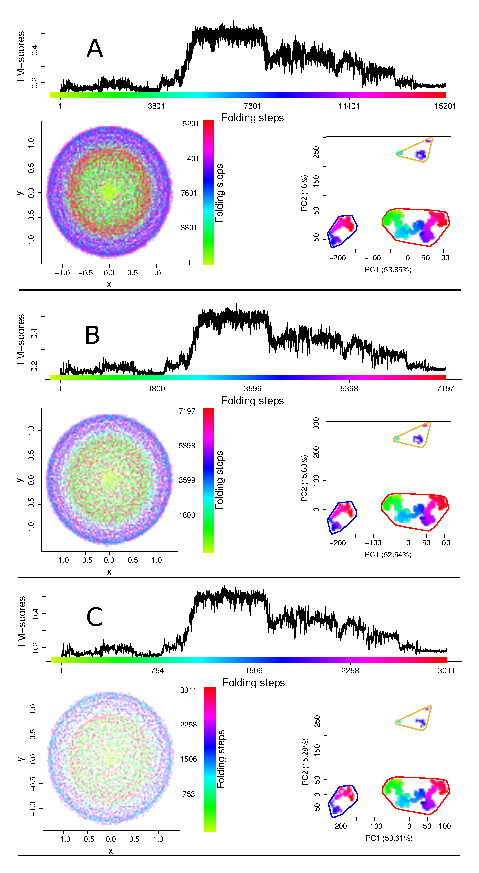
\includegraphics{images/06-paths-intrinsic-info}
\par\end{centering}
\caption{\csentence{Comparison with other methods.} Intrinsic information captured from the original trajectory of the villin-headpiece protein is largely preserved in the reduced trajectories produced by our algorithm. TM-score plot, nMDS pattern and clustering groups are presented at the top, bottom left, and bottom right of each panel. (A) Original trajectory. (B and C) Trajectories reduced by 52\% and 80\%, respectively. The nMDS produces a set of circular patterns associated with conformations occurring in different times of the simulation, whereas clustering produces a structure of three clusters associated with the first two principal components of the $C_{\alpha}$atoms of the conformations. \label{fig:Comparaciones-PCA-nMDS}}
\end{figure}


\subsection*{Algorithm performance}

The performance of the proposed algorithm was tested via two tests: a runtime comparison of the proposed algorithm with the three other typical techniques for folding reduction, i.e., nMDS, clustering, and PCA (Figure \ref{fig:Performance-methods}.A); and a parallel comparison in which the algorithm was run with several cores (Figure \ref{fig:Performance-methods}.B). For both tests, the trajectory corresponded to the first 100k conformations from the full trajectory of the \emph{trp-cage} protein, described above in Methods.

For the comparison among techniques (Figure \ref{fig:Performance-methods}.A), several subtrajectories of different lengths were reduced by all the techniques. When the techniques were run with one core, PCA showed the most efficient runtimes, followed by our proposed algorithm, whereas nMDS and clustering became impractical when used with short to medium trajectories. Furthermore, in contrast to the other techniques, the proposed algorithm has the advantage of being able to run easily in parallel. When it was run using two cores, the runtime was reduced by half and was shorter than that achieved with PCA.

\begin{figure}[th]
\begin{centering}
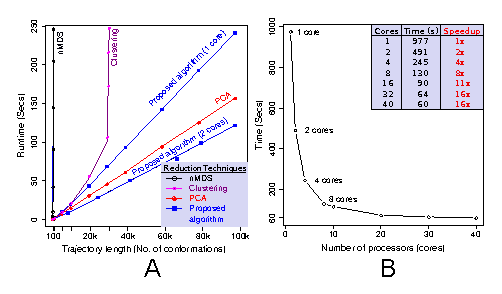
\includegraphics{images/07-performance-times}
\par\end{centering}
\caption{\csentence{Performance of the algorithm.} (A) Runtime comparisons for four folding reduction techniques: nMDS, clustering, PCA, and our proposed algorithm (running with one and two cores). With one core, PCA was the most efficient algorithm, followed by our algorithm. However, when the proposed algorithm was run with two cores, its runtime was reduced by half, being more efficient than PCA. (B) Evaluation of algorithm parallelization. When the number of processing cores is multiplied by two, the processing time reduces by half with a quasi-linear speedup that is maintained for up to \textasciitilde{}8 cores (8x). \label{fig:Performance-methods}\protect \\
}
\end{figure}

To test how parallelization improves the algorithm performance, the full dataset of 100k conformations was reduced by the algorithm using a different number of cores. The runtimes are shown in Figure \ref{fig:Performance-methods}.B, which reveals a good acceleration, with the processing time reduced by half with every doubling of core number. This speedup is maintained up to \textasciitilde{}8 cores and decreases to a minimum after \textasciitilde{}30 cores.

These results show that the algorithm has good performance compared with that of the other techniques and that this performance is improved when the algorithm is run in parallel using more than one core. As a consequence, the speedup of the algorithm scales quasilinearly with the number of processing cores to almost 8x, and with 32 cores, the algorithm achieves a speedup of 16x. Considering that multicore technology is commonplace even for desktop computers, the proposed algorithm has the capacity to take advantage of this technology to reduce large protein folding trajectories in a fast parallel manner, with runtimes closer or better than those of other techniques commonly used for this task.

\section*{Conclusions}

Although the progress in long timescale simulations of protein folding has enabled the generation of large folding trajectories, a new challenge lies in their analysis. Due to the millions of conformations they can contain, their processing and analysis is difficult or impractical.

Here, we have proposed a fast and parallel algorithm to simplify large protein-folding trajectories. The algorithm reduces a trajectory by splitting it into segments and then reducing each in parallel using a fast clustering strategy that avoids the pairwise comparison of all structures.

According to the results, our algorithm can summarize a folding trajectory with high data compression and preserve its main conformations and intrinsic information. This was confirmed by comparing the patterns and groups obtained in the original trajectory and the reduced trajectories through the use of nMDS and clustering techniques. Besides, the algorithm runtime shows a linear trend with a performance close to that of PCA, the technique with the best performance among the three evaluated in this work. And, when the algorithm utilizes two or more processing cores, its performance is much better, with quasi-linear acceleration maintained up to \textasciitilde{}8 cores (8x).

Nevertheless, the proposed algorithm is limited to creating a summary of the main events of a protein folding trajectory without performing any kind of analysis, as other techniques do, such as nMDS and clustering However, these summarized trajectories can be used as input to these and other techniques that serve the same purpose and but which were not designed to handle large protein- folding trajectories.

\section*{Availability and requirements}
\begin{itemize}
\item \textbf{Project~name:} FastFoldingReduction
\item \textbf{Operating~System}: Platform-independent
\item \textbf{Programming~Languajes}: R and Fortran (Source code to work with many OS systems)
\item \textbf{License}: GNU GPL
\end{itemize}
\begin{backmatter}

\section*{Acknowledgements}

The authors would like to thank the Bioinformatics research group at Universidad del Valle for use of the computer facilities. The authors would also like to thank D.E. Shaw Research for providing the all-atom Molecular Dynamics simulation data. 

\section*{Authors’ contributions }

LG and MM designed the algorithm. LG implemented the algorithm and wrote the manuscript. NM carried out the data collection and analysis. PM guided the study and helped to draft the manuscript. All authors read and approved the final manuscript.

\bibliographystyle{bmc_mathphys}
\bibliography{paperBMC_references}

\end{backmatter}
\end{document}
\end{document}
